% Appendix A

\chapter{Systematic studies follow-up}

%----------------------------------------------------------------------------------------

\section{Systematic uncertainty associated with the RICH}

\begin{figure}[!p]
  \centering
	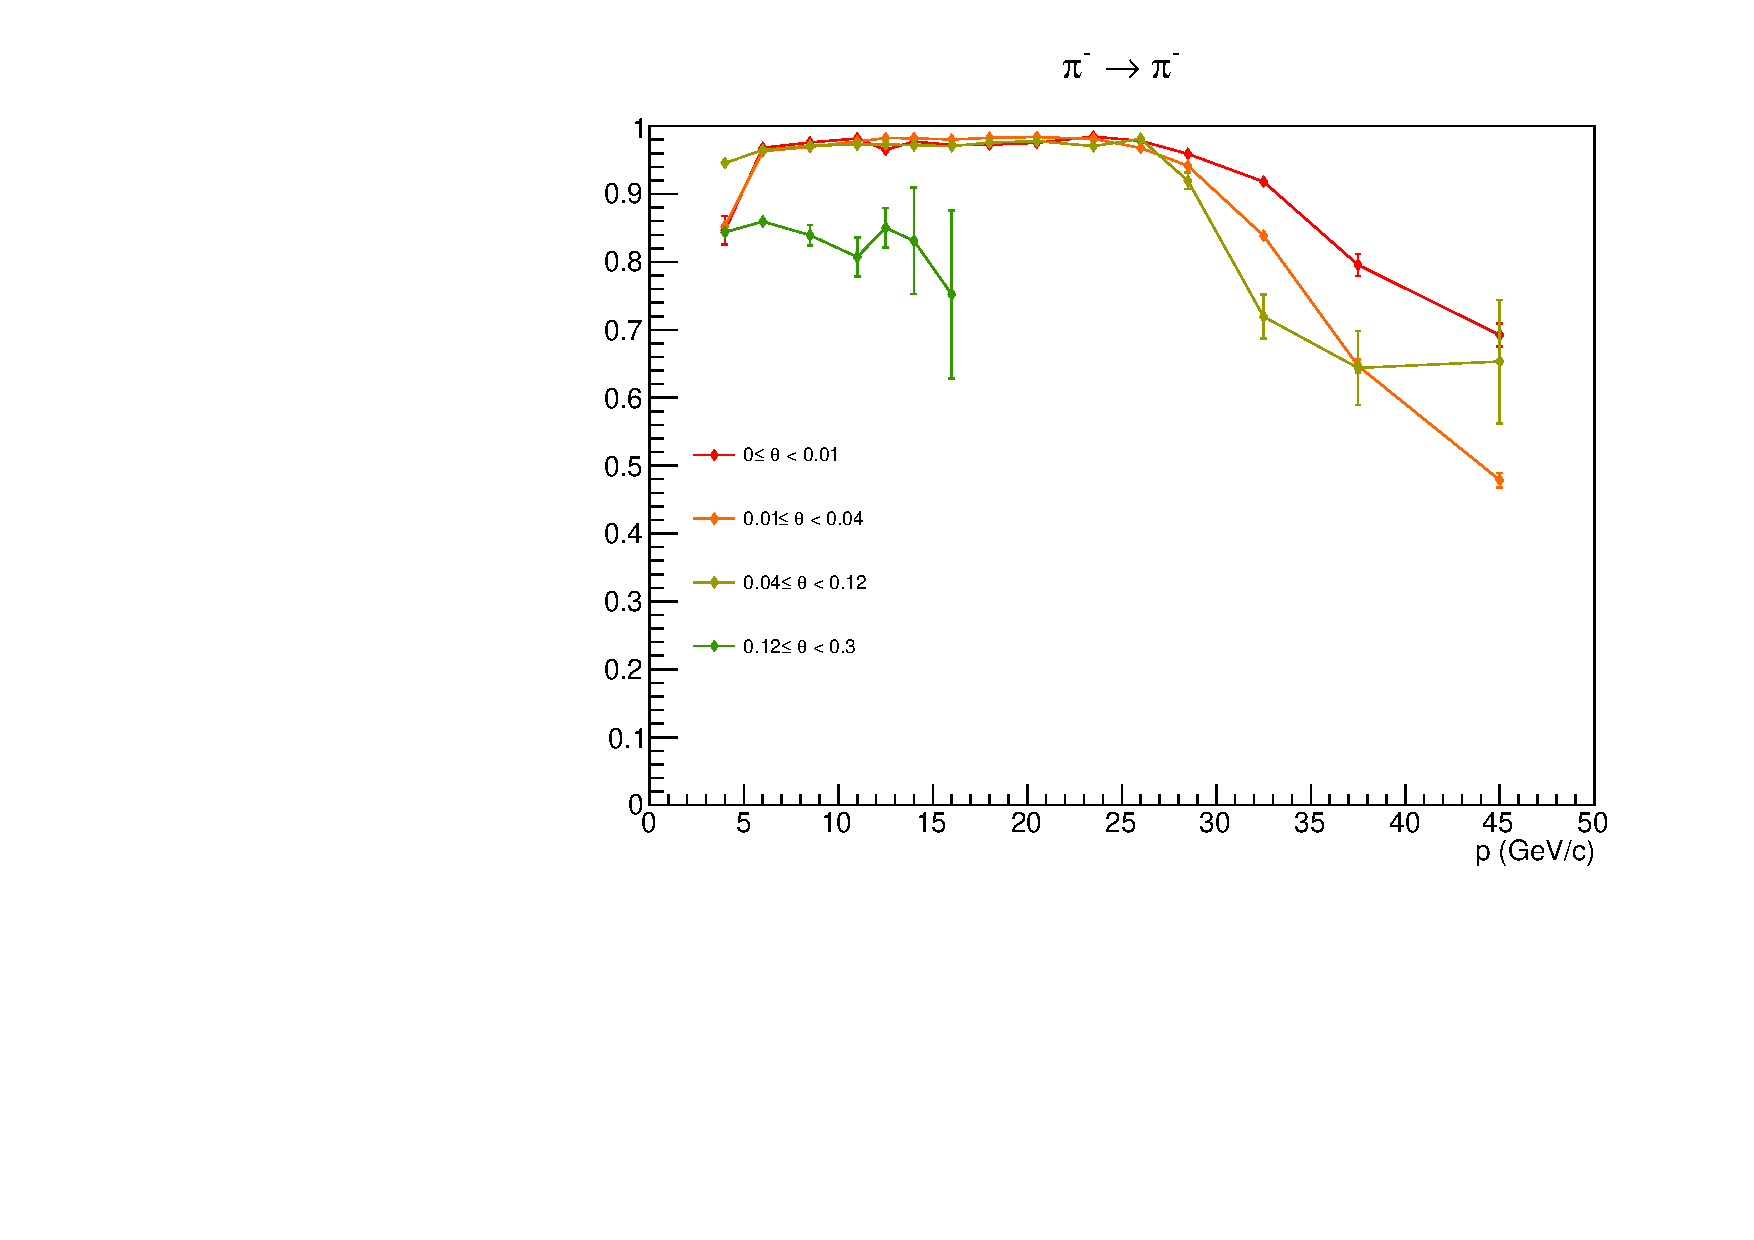
\includegraphics[scale=0.38]{./gfx/pim_pi.pdf}
  \includegraphics[scale=0.38]{./gfx/pim_K.pdf}
  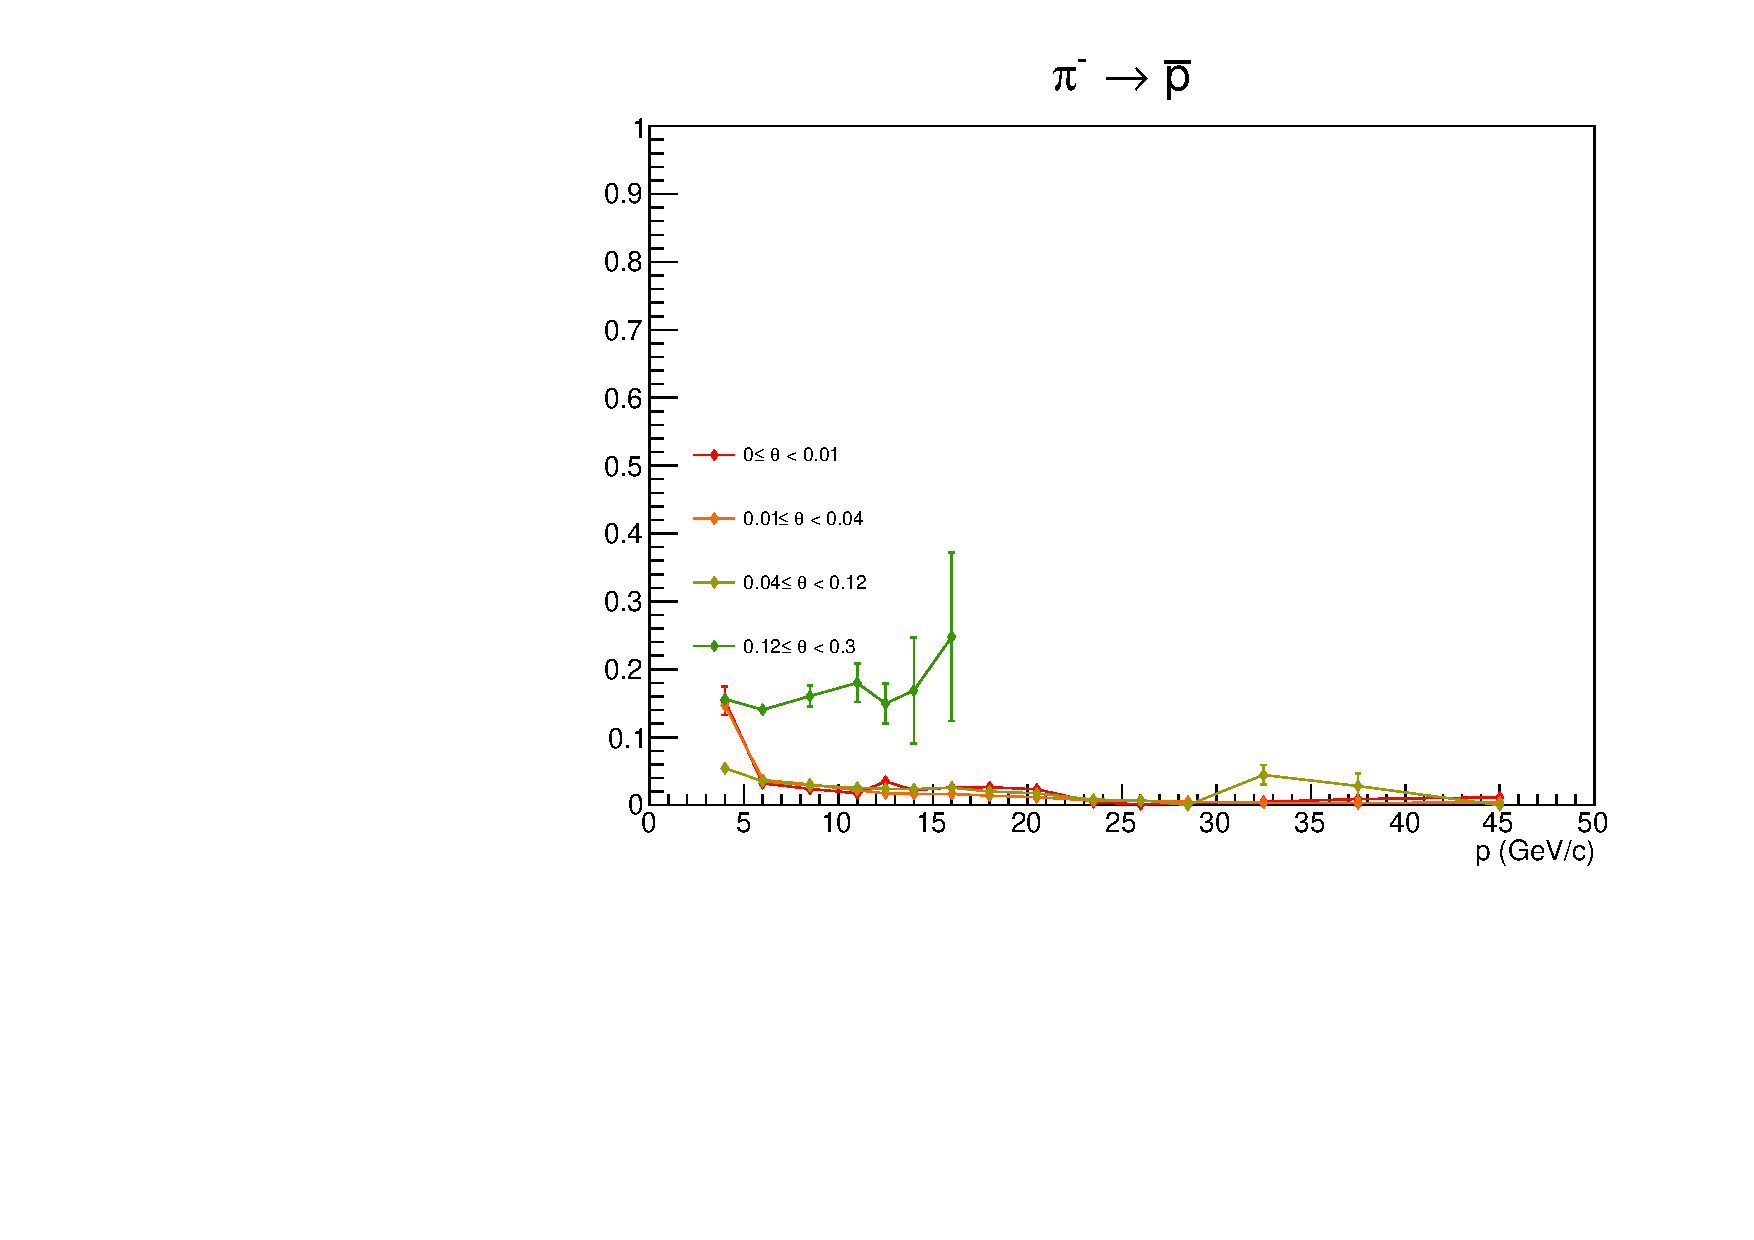
\includegraphics[scale=0.38]{./gfx/pim_p.pdf}
  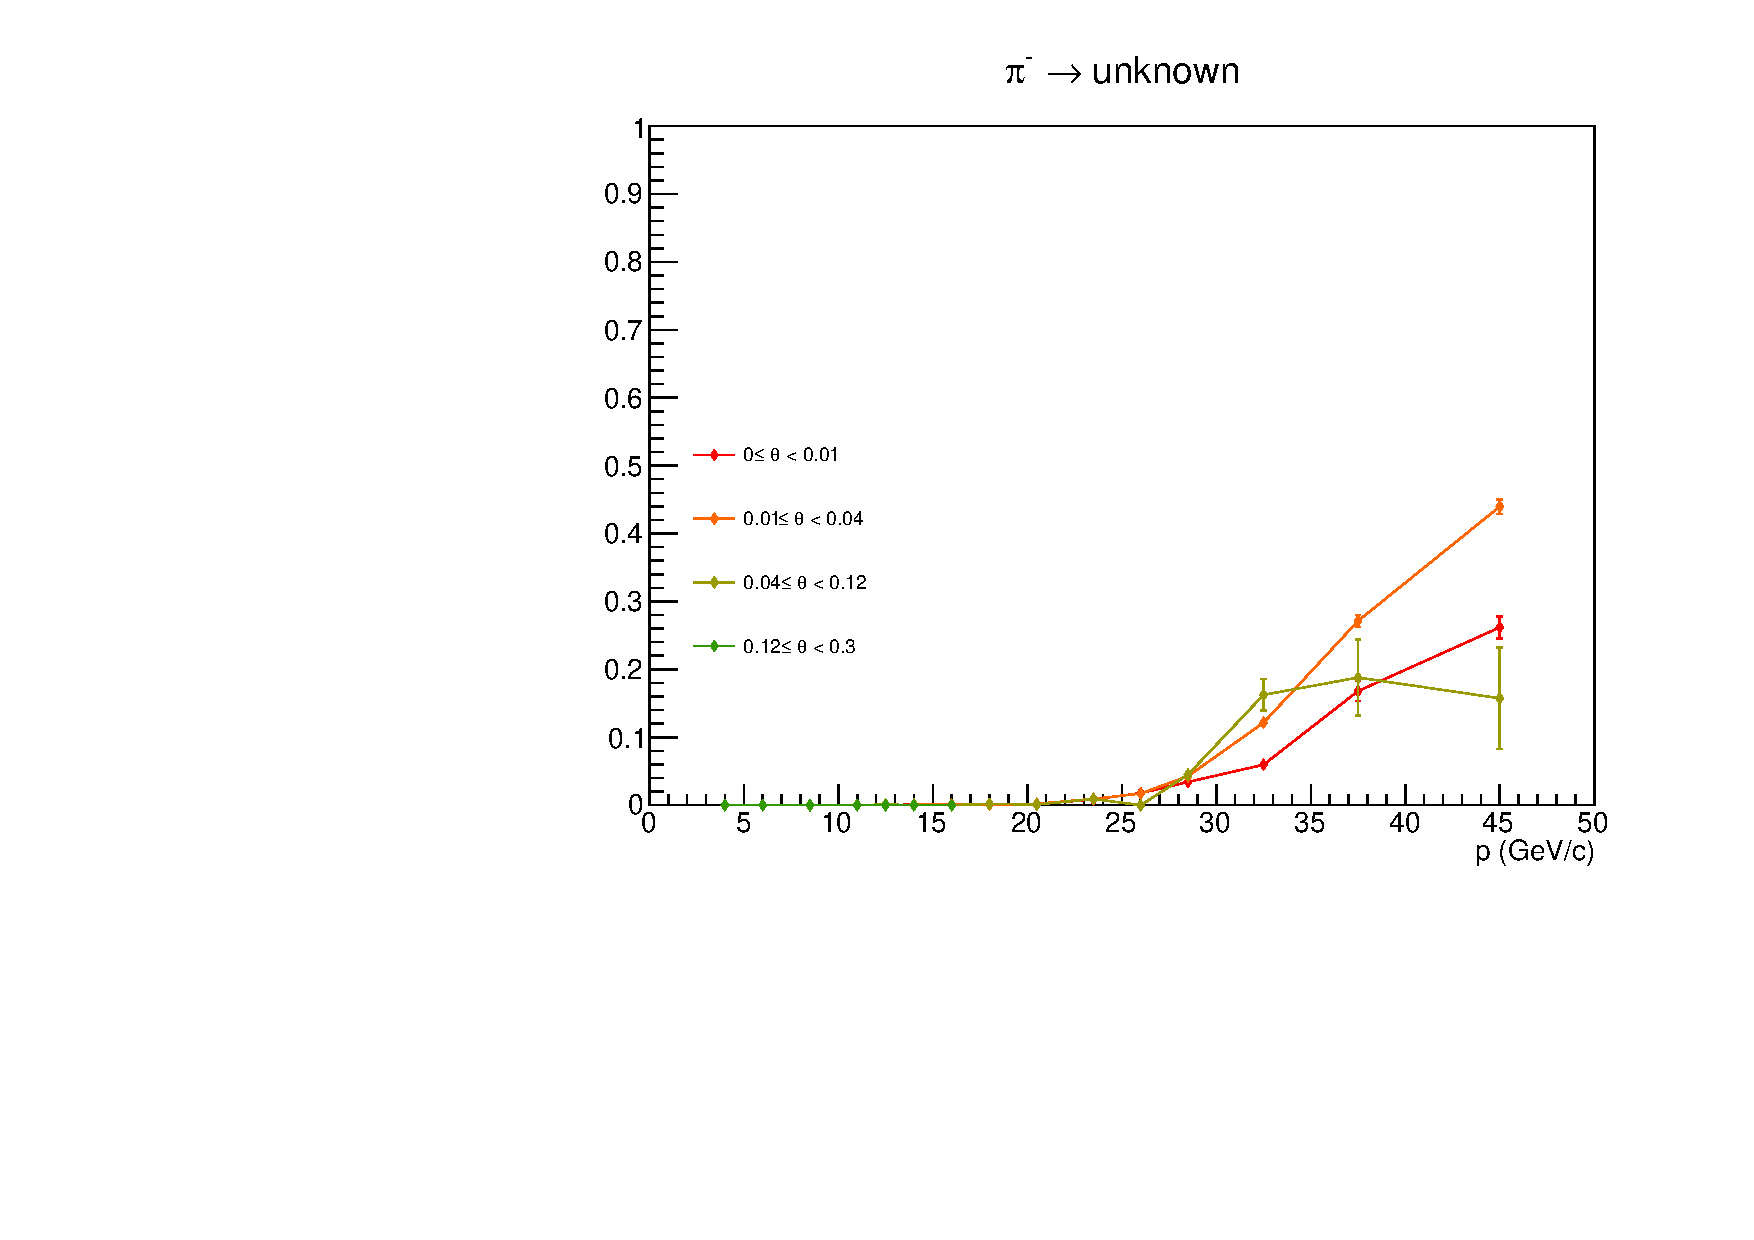
\includegraphics[scale=0.38]{./gfx/pim_u.pdf}
	\caption{Identification probabilities $\epsilon(p \rightarrow j)$ for $\pi^-$.}
	\label{pic:Effpim}
\end{figure}


\begin{figure}[!p]
  \centering
	\includegraphics[scale=0.38]{./gfx/Km_pi.pdf}
  \includegraphics[scale=0.38]{./gfx/Km_K.pdf}
  \includegraphics[scale=0.38]{./gfx/Km_p.pdf}
  \includegraphics[scale=0.38]{./gfx/Km_u.pdf}
	\caption{Identification probabilities $\epsilon(p \rightarrow j)$ for $K^-$.}
	\label{pic:Effkm}
\end{figure}

\begin{figure}[!p]
  \centering
	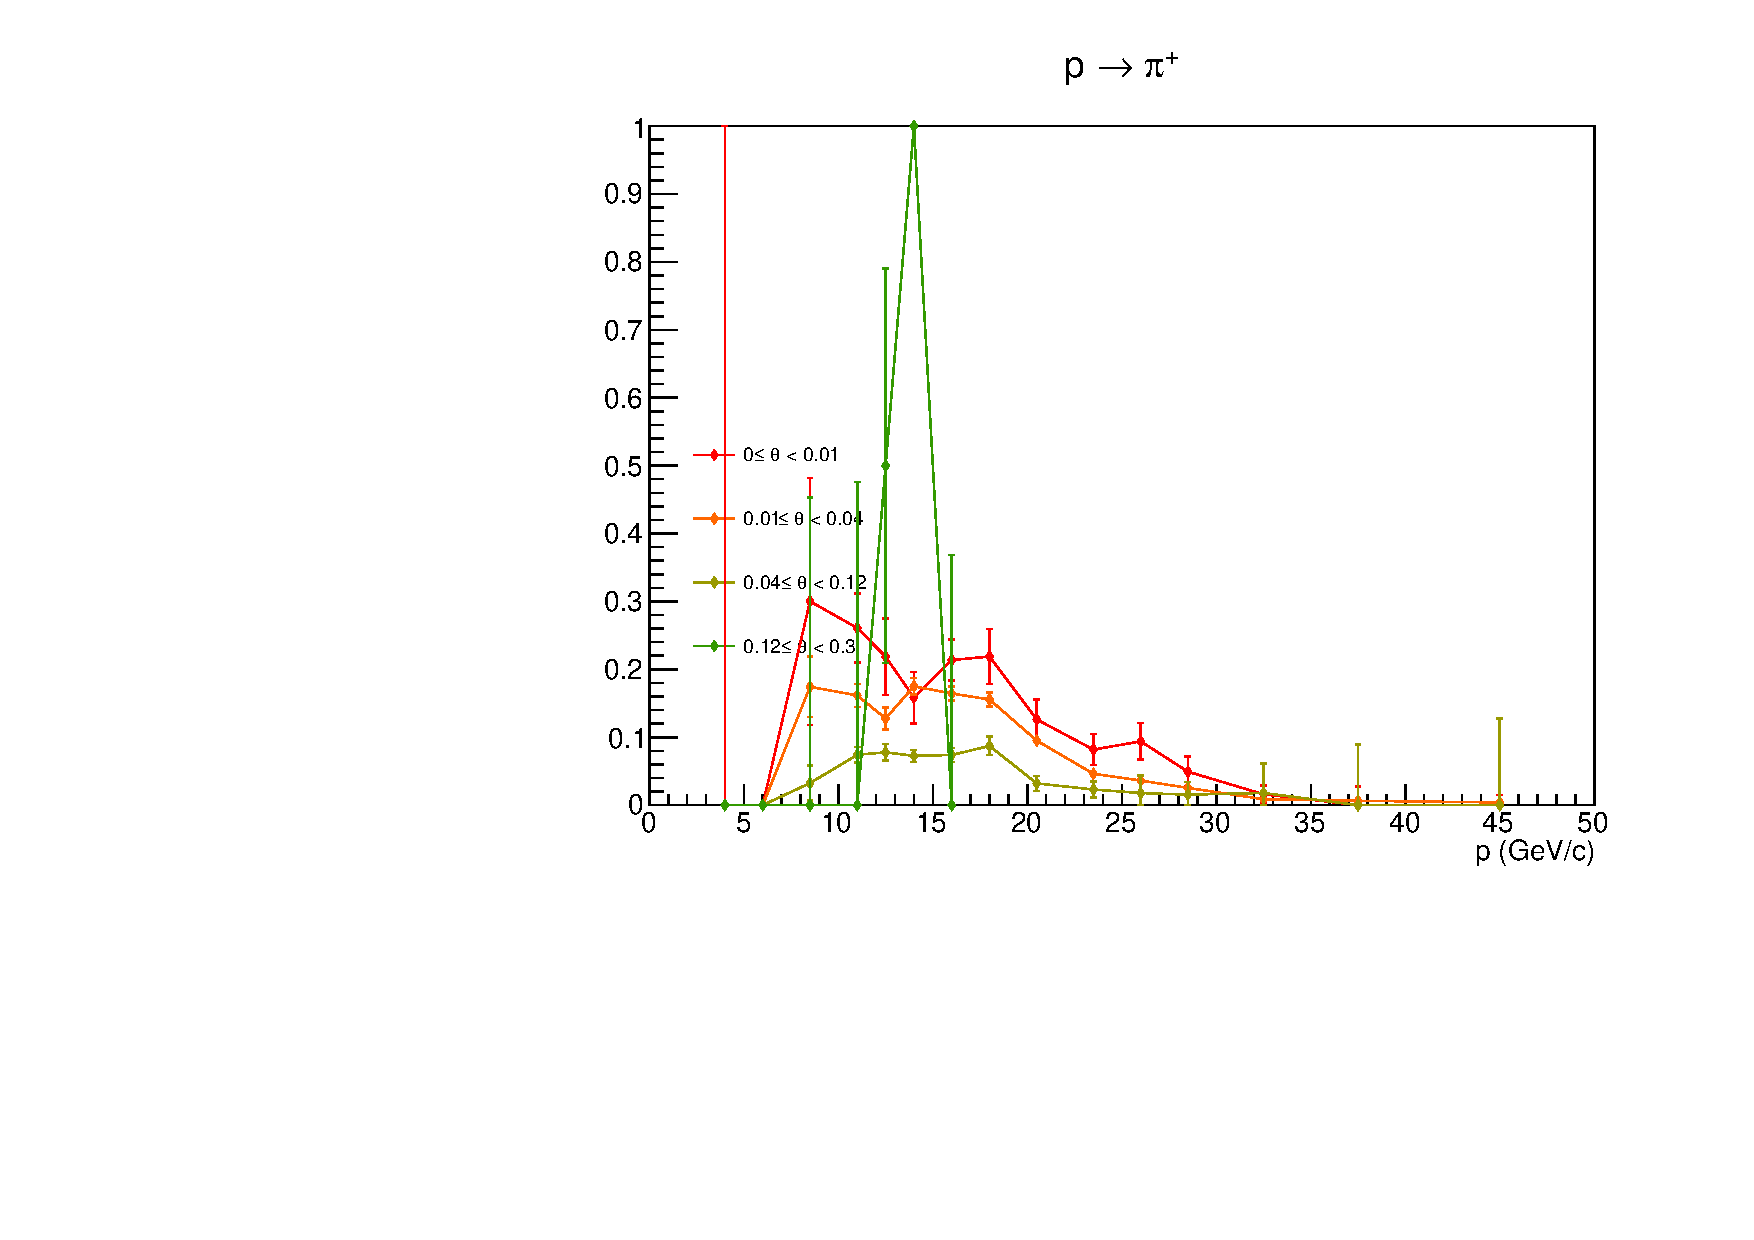
\includegraphics[scale=0.38]{./gfx/pp_pi.pdf}
  \includegraphics[scale=0.38]{./gfx/pp_K.pdf}
  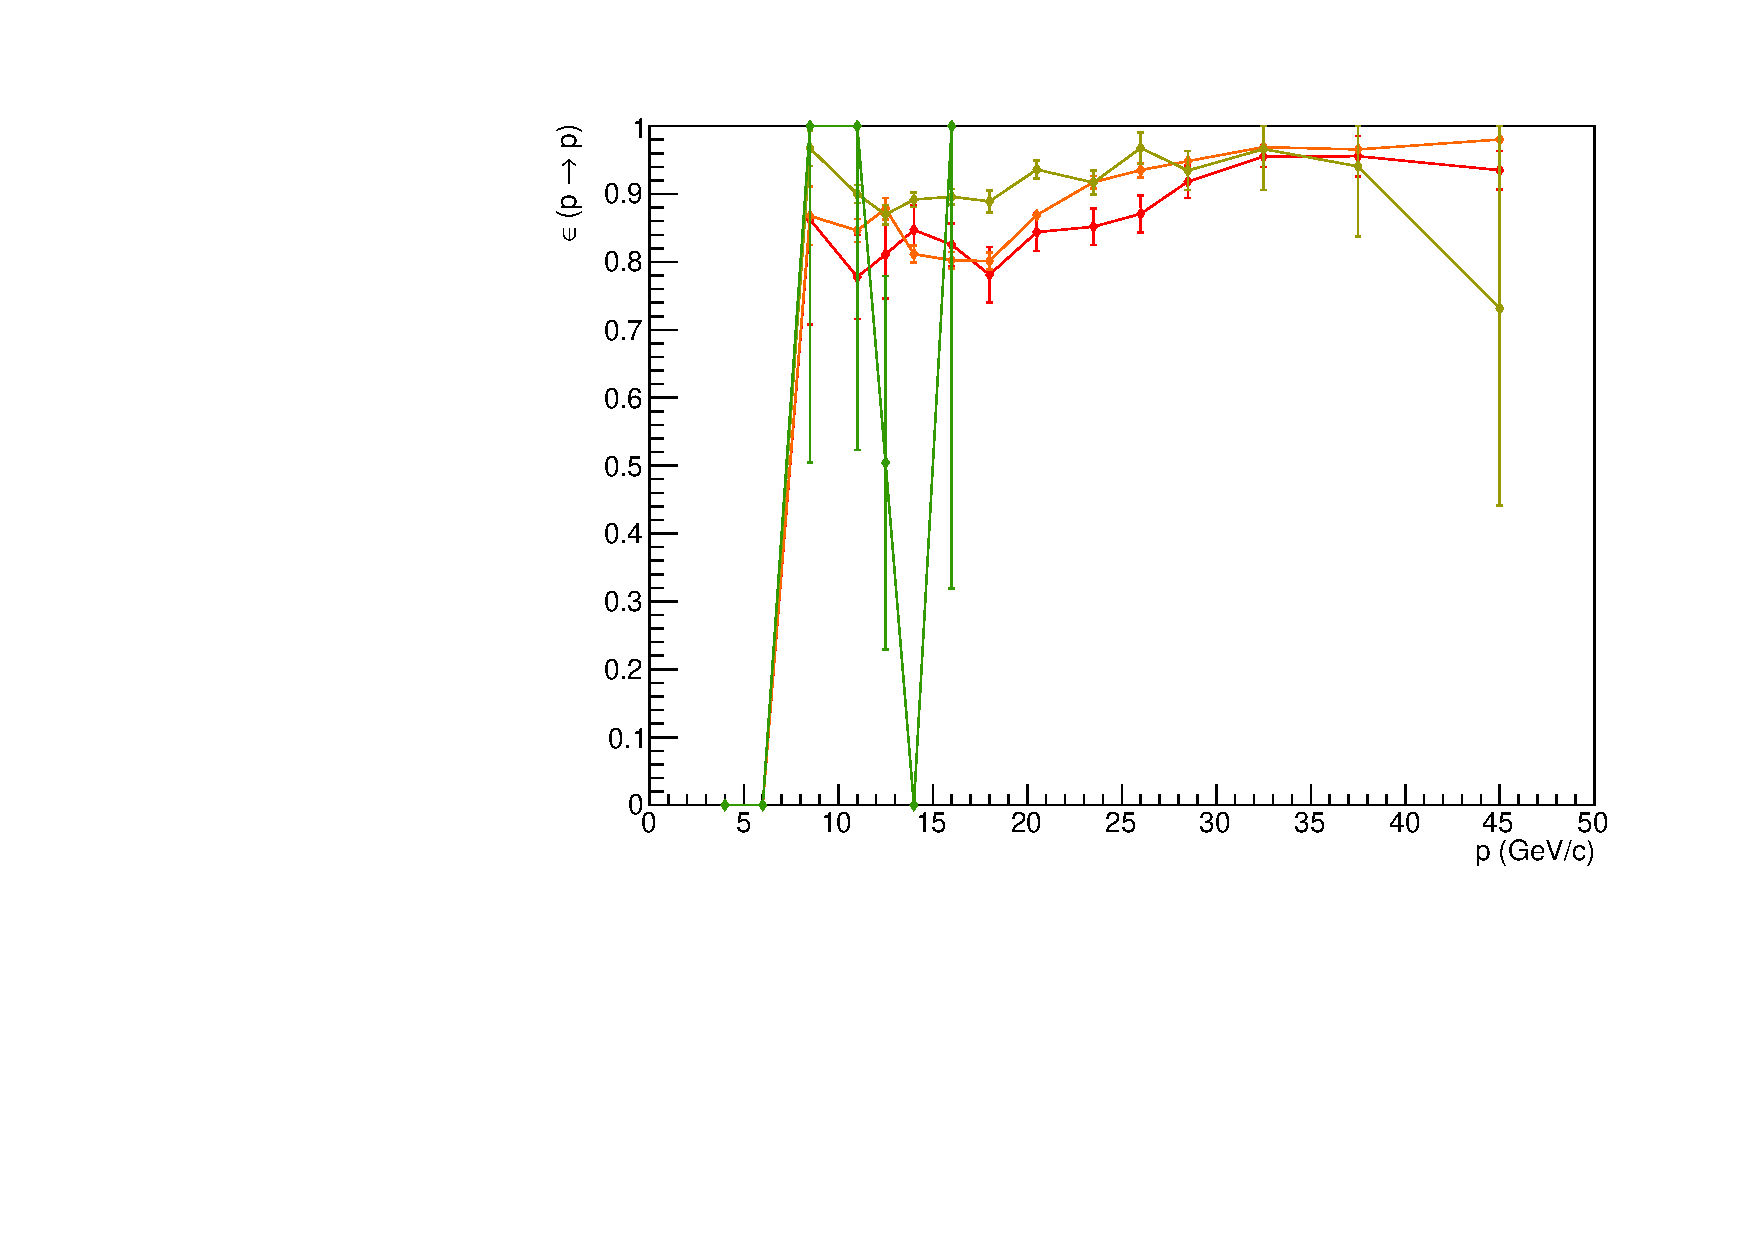
\includegraphics[scale=0.38]{./gfx/pp_p.pdf}
  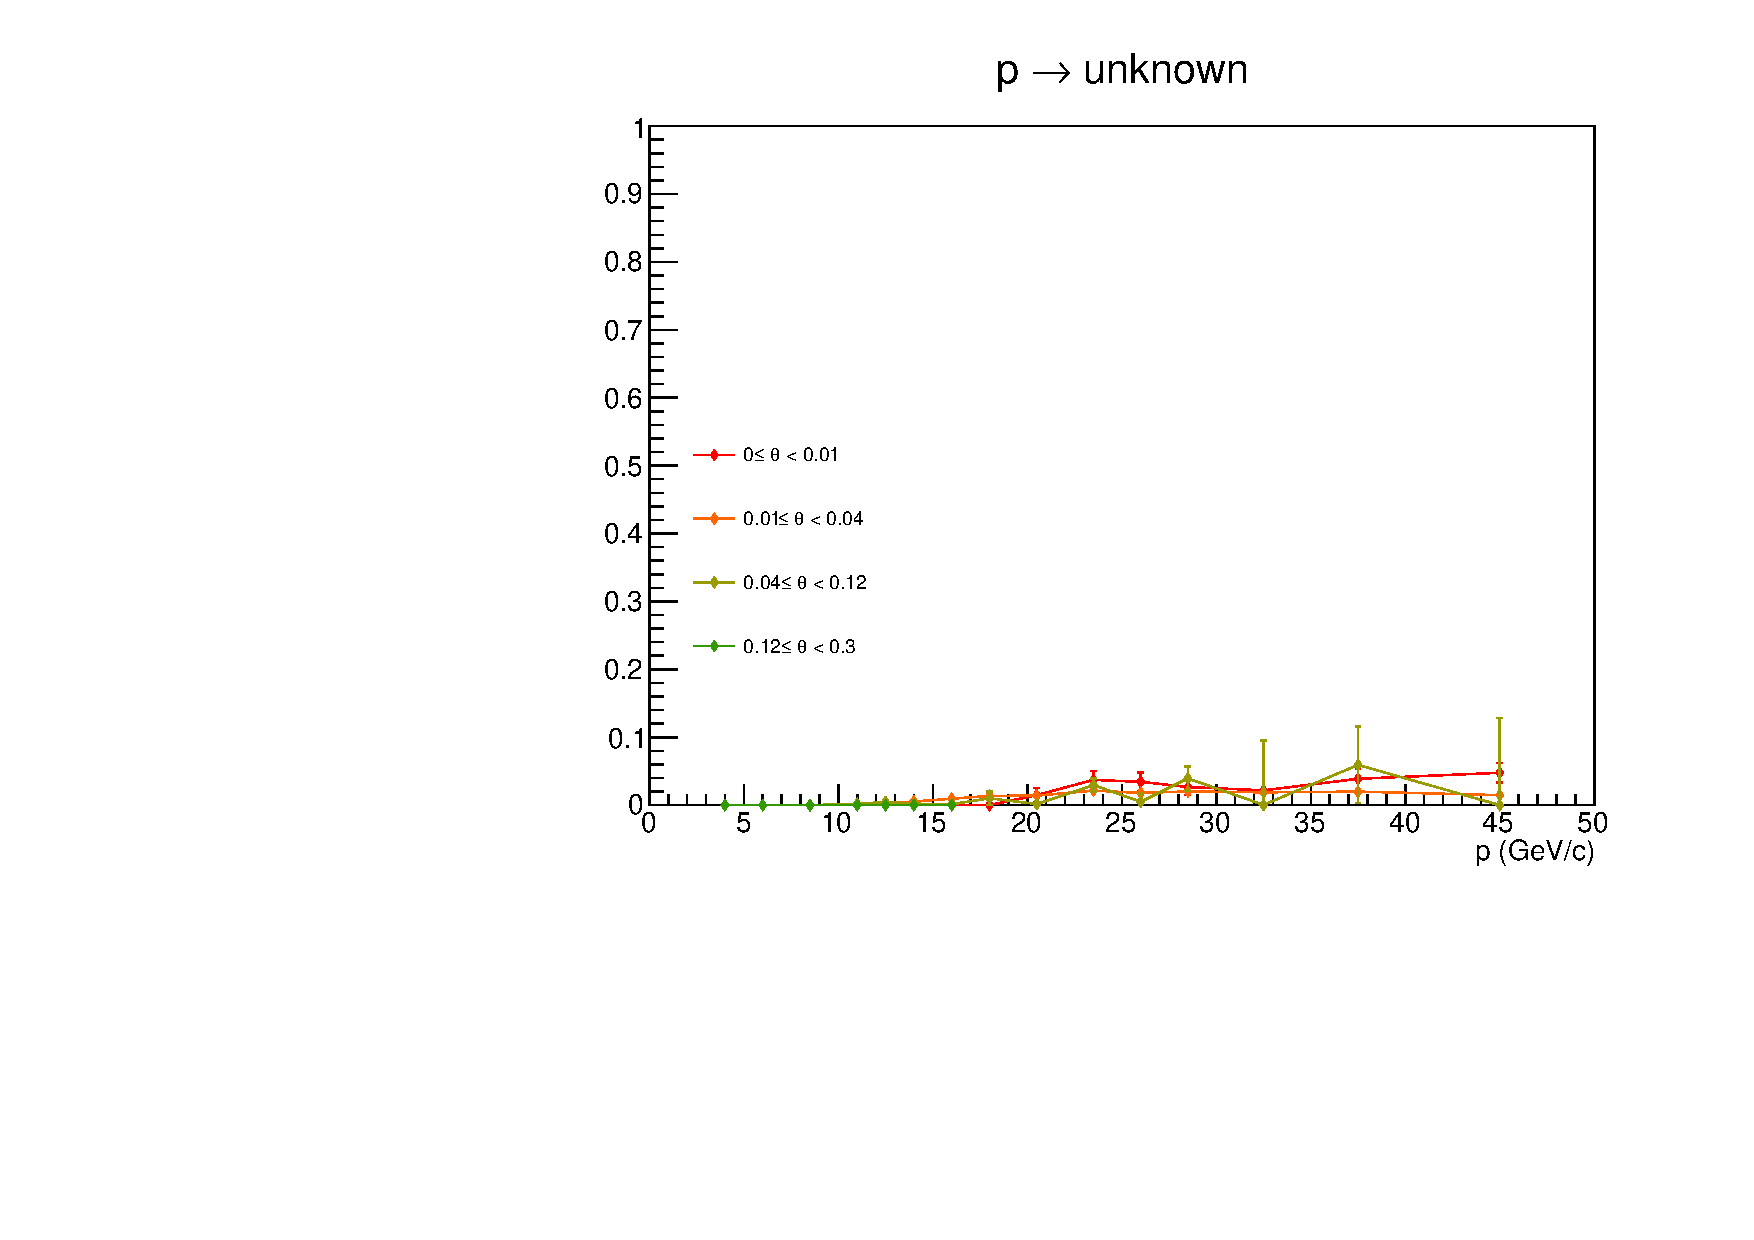
\includegraphics[scale=0.38]{./gfx/pp_u.pdf}
	\caption{Identification probabilities $\epsilon(p \rightarrow j)$ for $p$.}
	\label{pic:Effpp}
\end{figure}

\begin{figure}[!p]
  \centering
	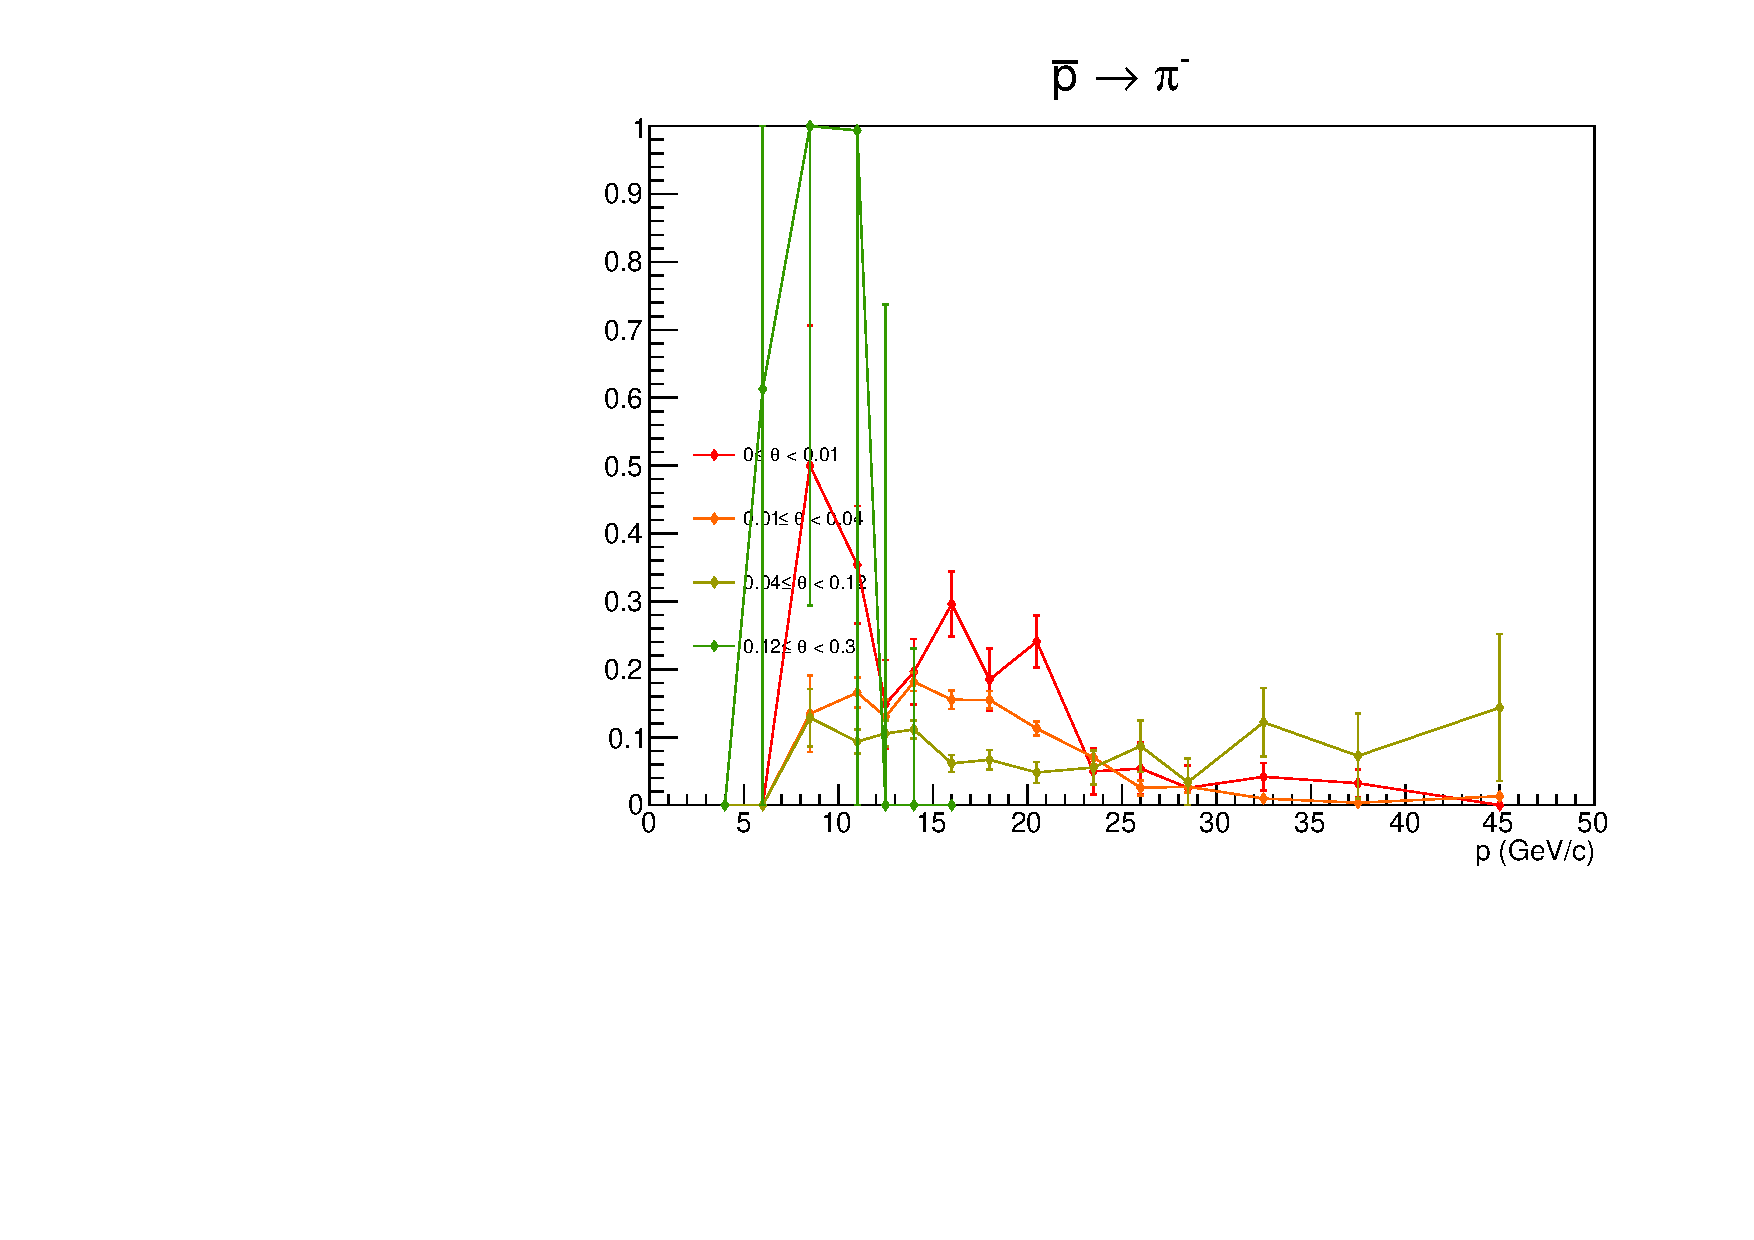
\includegraphics[scale=0.38]{./gfx/pm_pi.pdf}
  \includegraphics[scale=0.38]{./gfx/pm_K.pdf}
  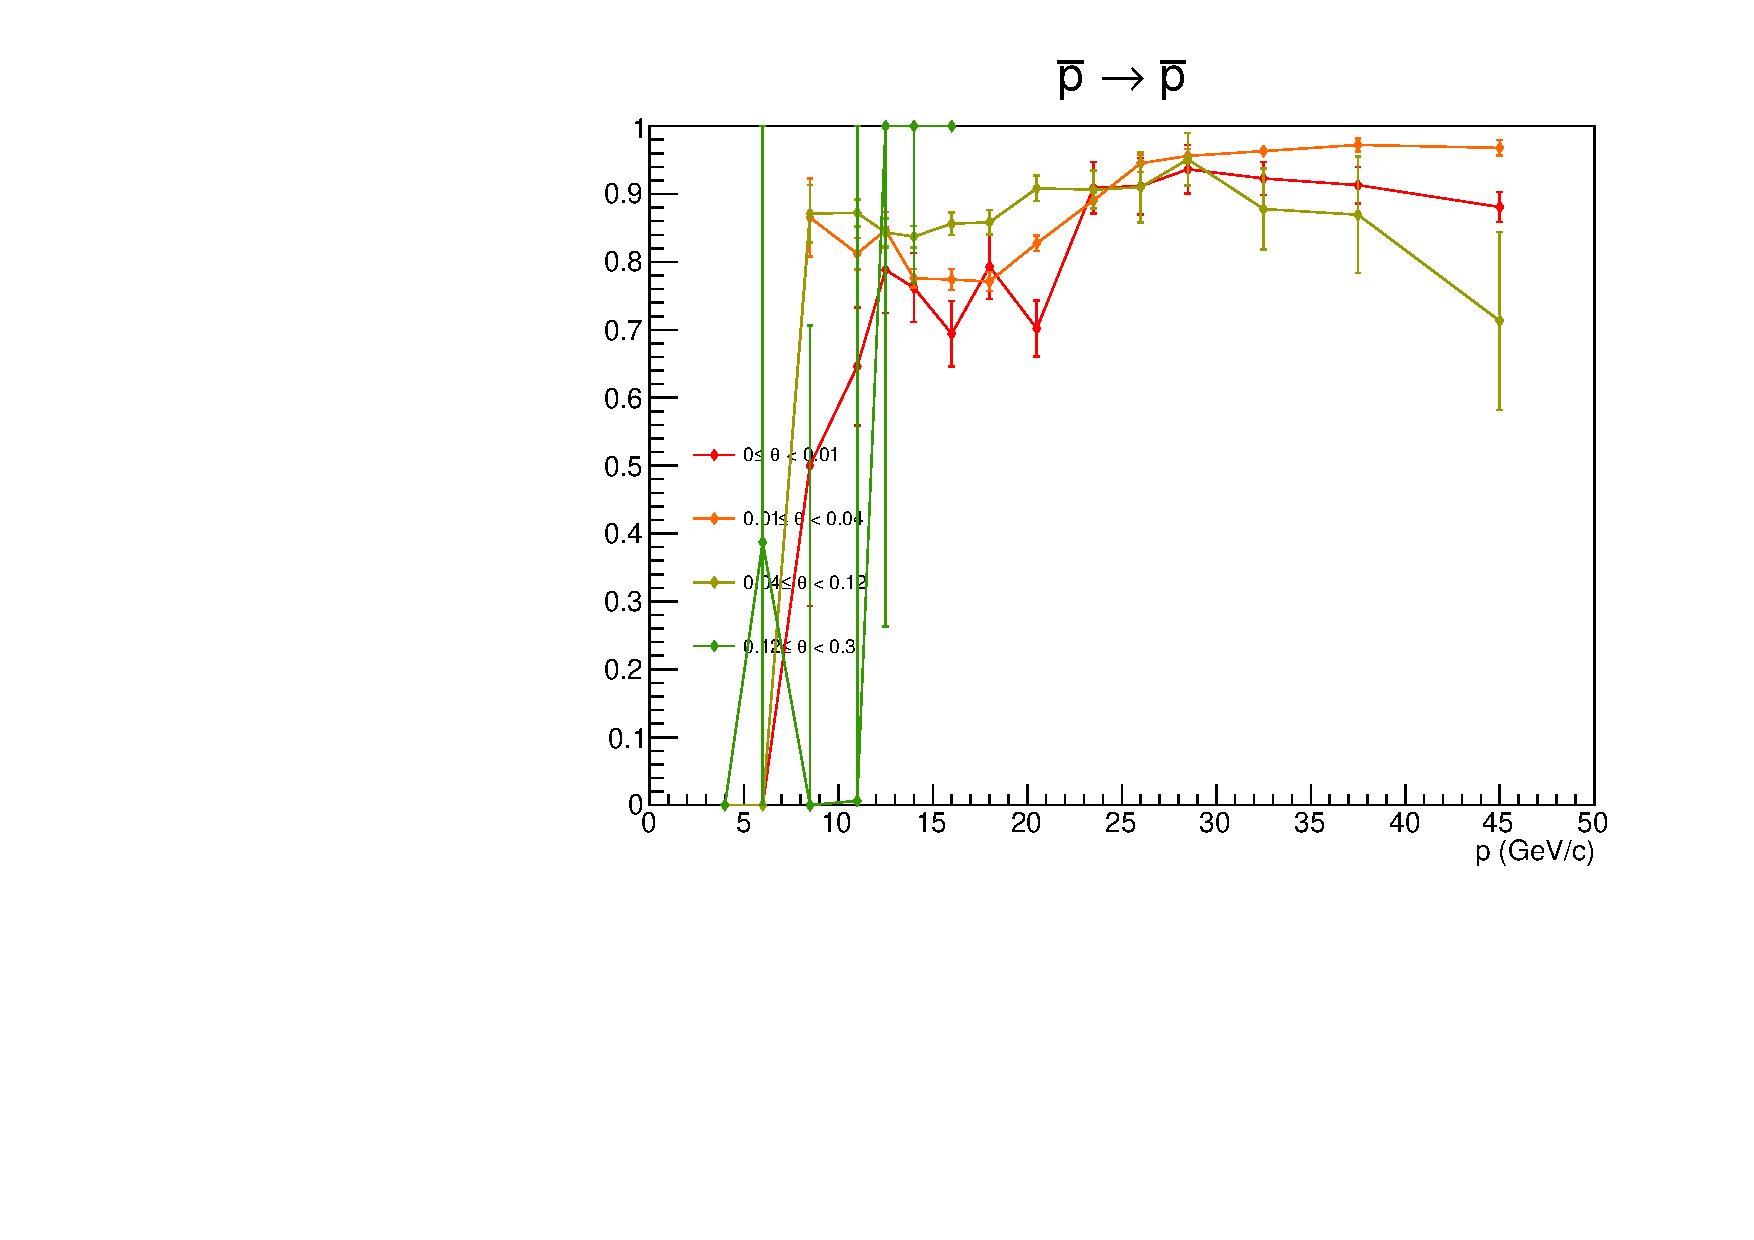
\includegraphics[scale=0.38]{./gfx/pm_p.pdf}
  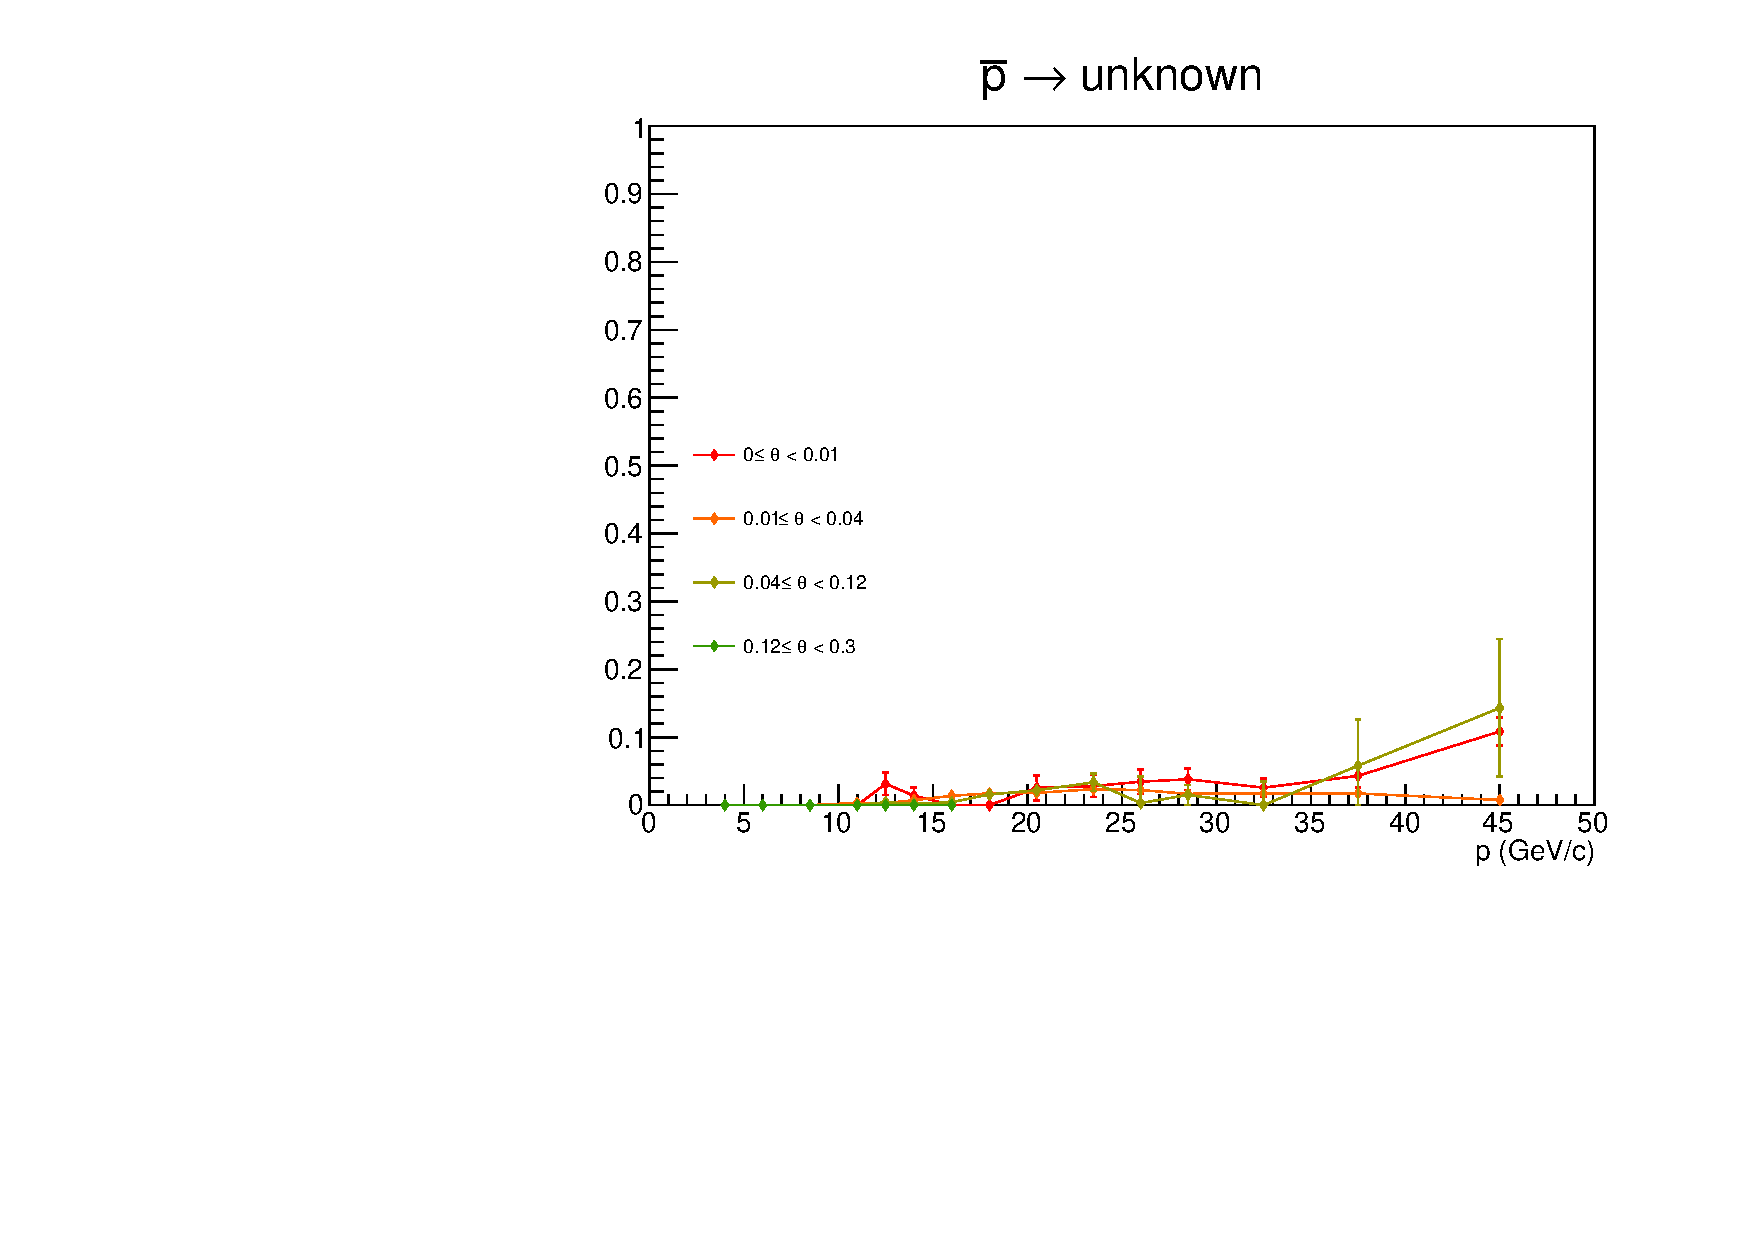
\includegraphics[scale=0.38]{./gfx/pm_u.pdf}
	\caption{Identification probabilities $\epsilon(p \rightarrow j)$ for $\bar{p}$.}
	\label{pic:Effpm}
\end{figure}


%----------------------------------------------------------------------------------------

\section{Systematic uncertainty associated to the stability of data over time}

\begin{sidewaysfigure}[p]
  \centering
	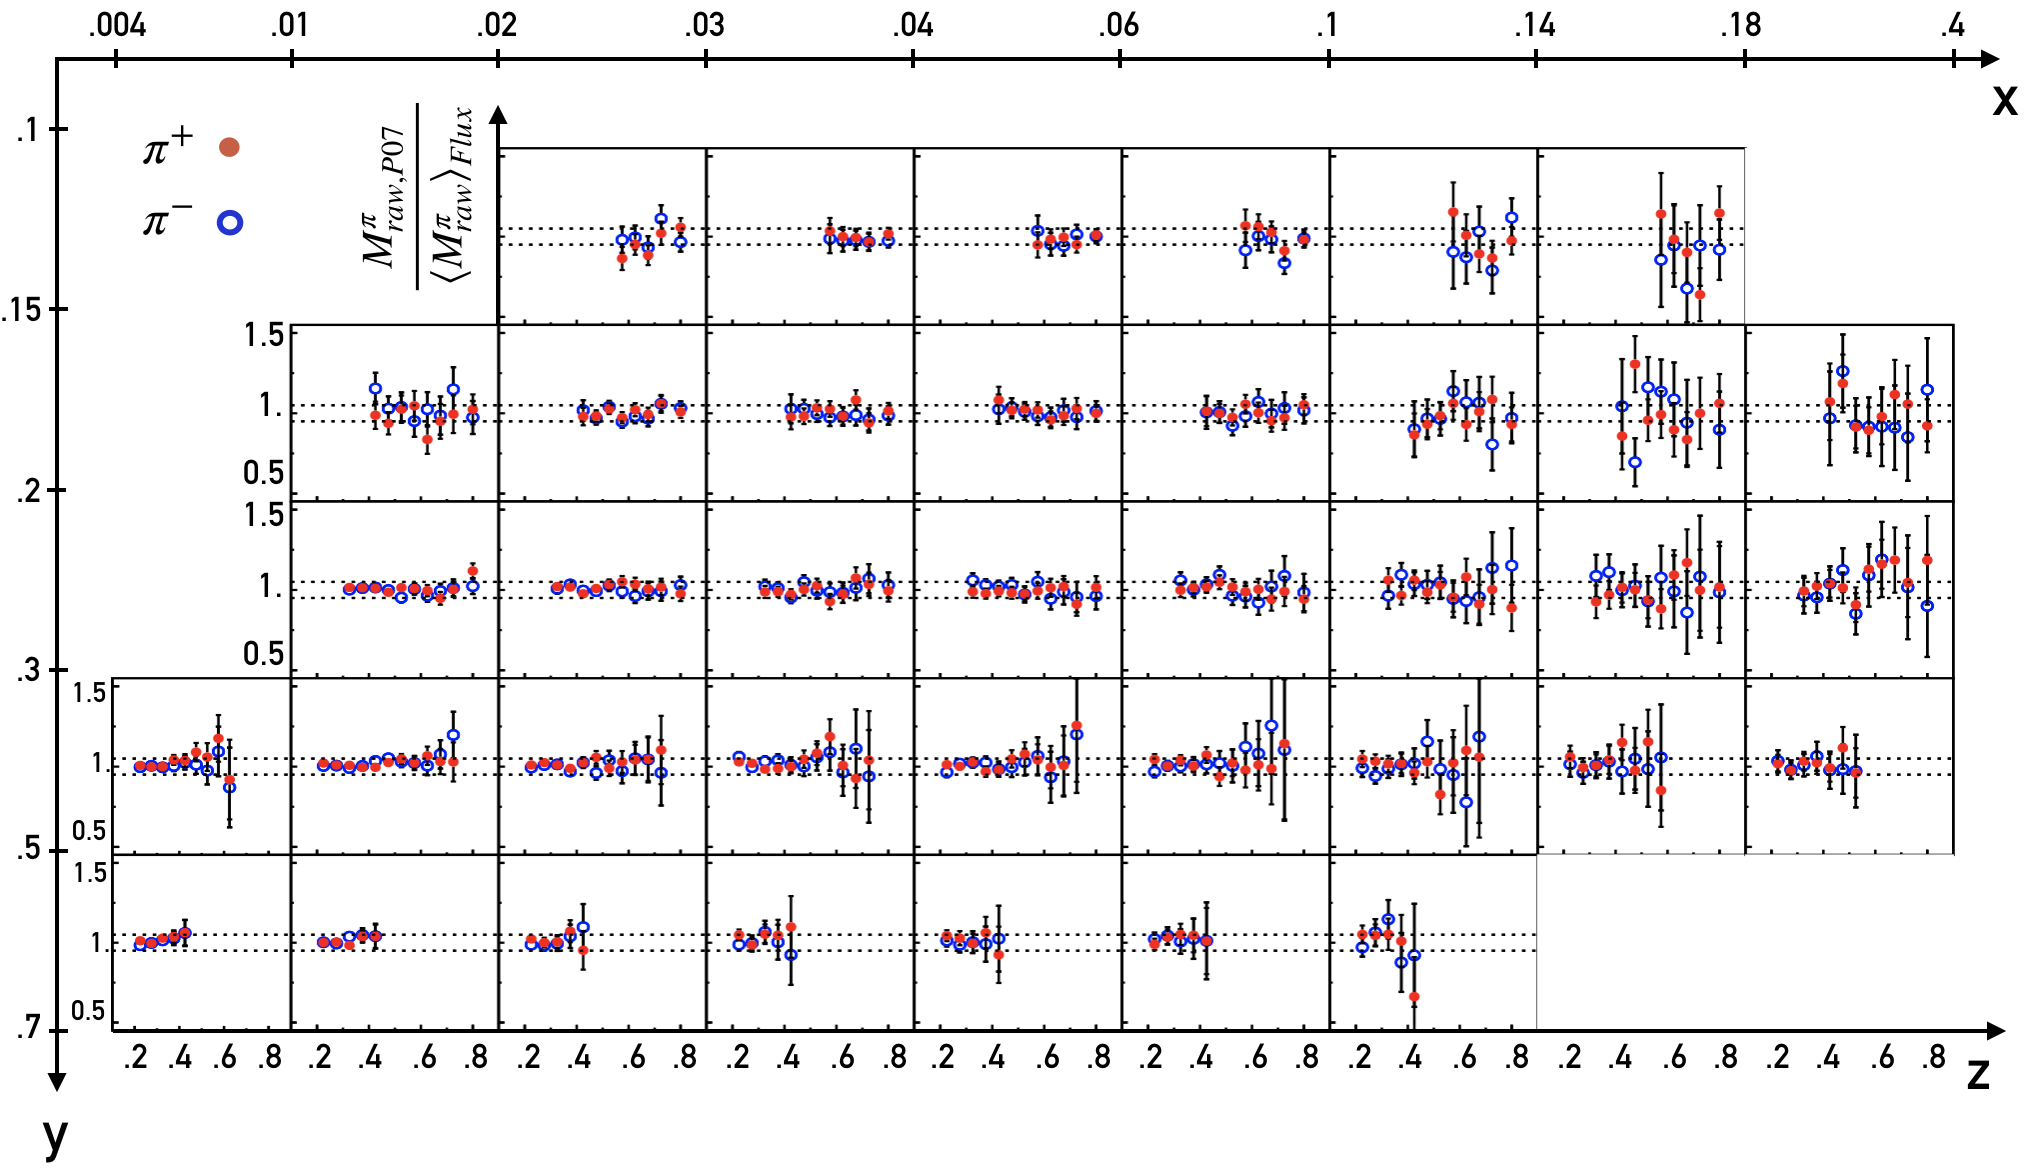
\includegraphics[scale=0.7]{./gfx/SysTimeMultpi.png}
	\caption{Same as Fig. \ref{pic:hMultTime} but for pion multiplicities.}
	\label{pic:piMultTime}
\end{sidewaysfigure}

\begin{sidewaysfigure}[p]
  \centering
	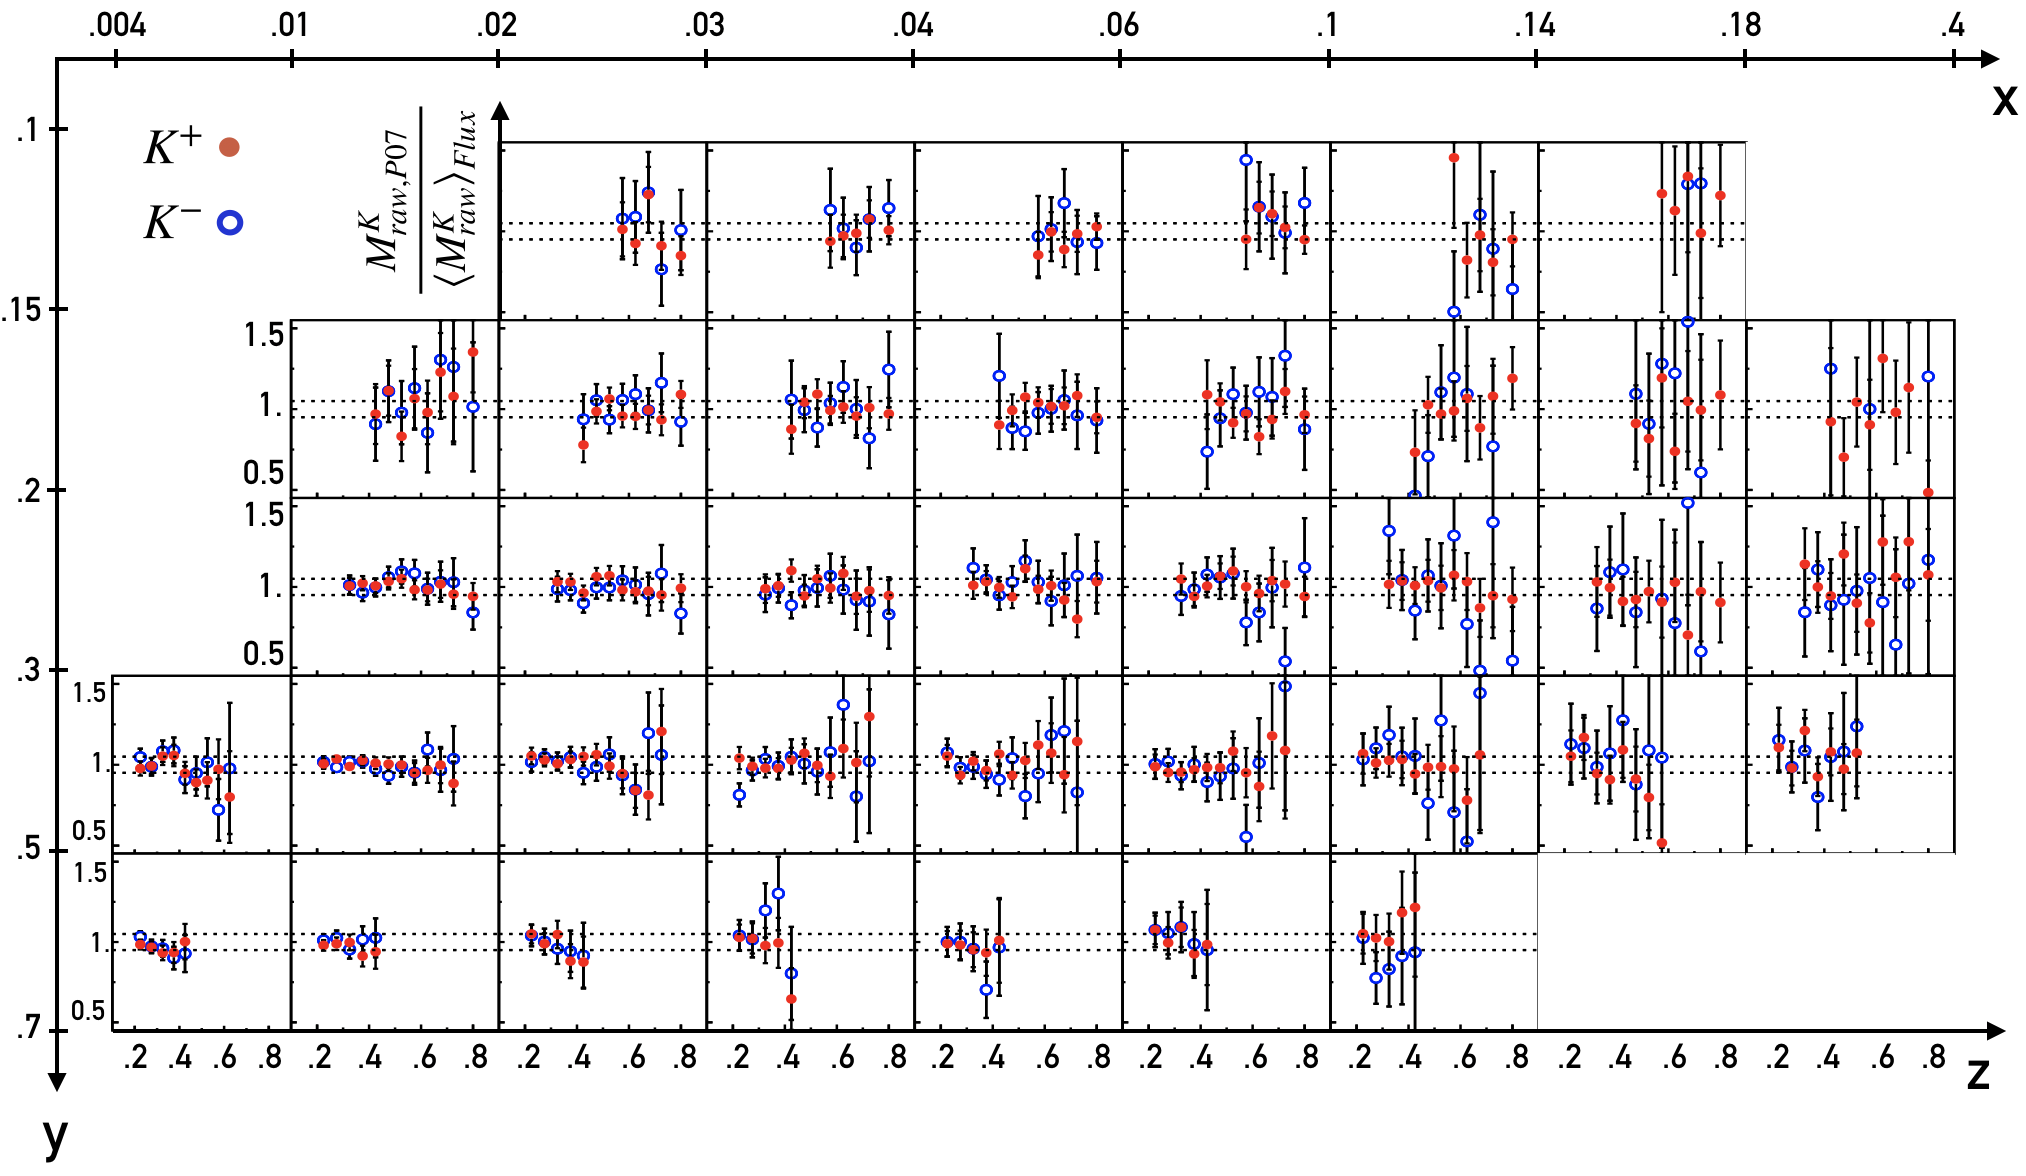
\includegraphics[scale=0.7]{./gfx/SysTimeMultk.png}
	\caption{Same as Fig. \ref{pic:hMultTime} but for kaon multiplicities.}
	\label{pic:kMultTime}
\end{sidewaysfigure}

\begin{sidewaysfigure}[p]
  \centering
	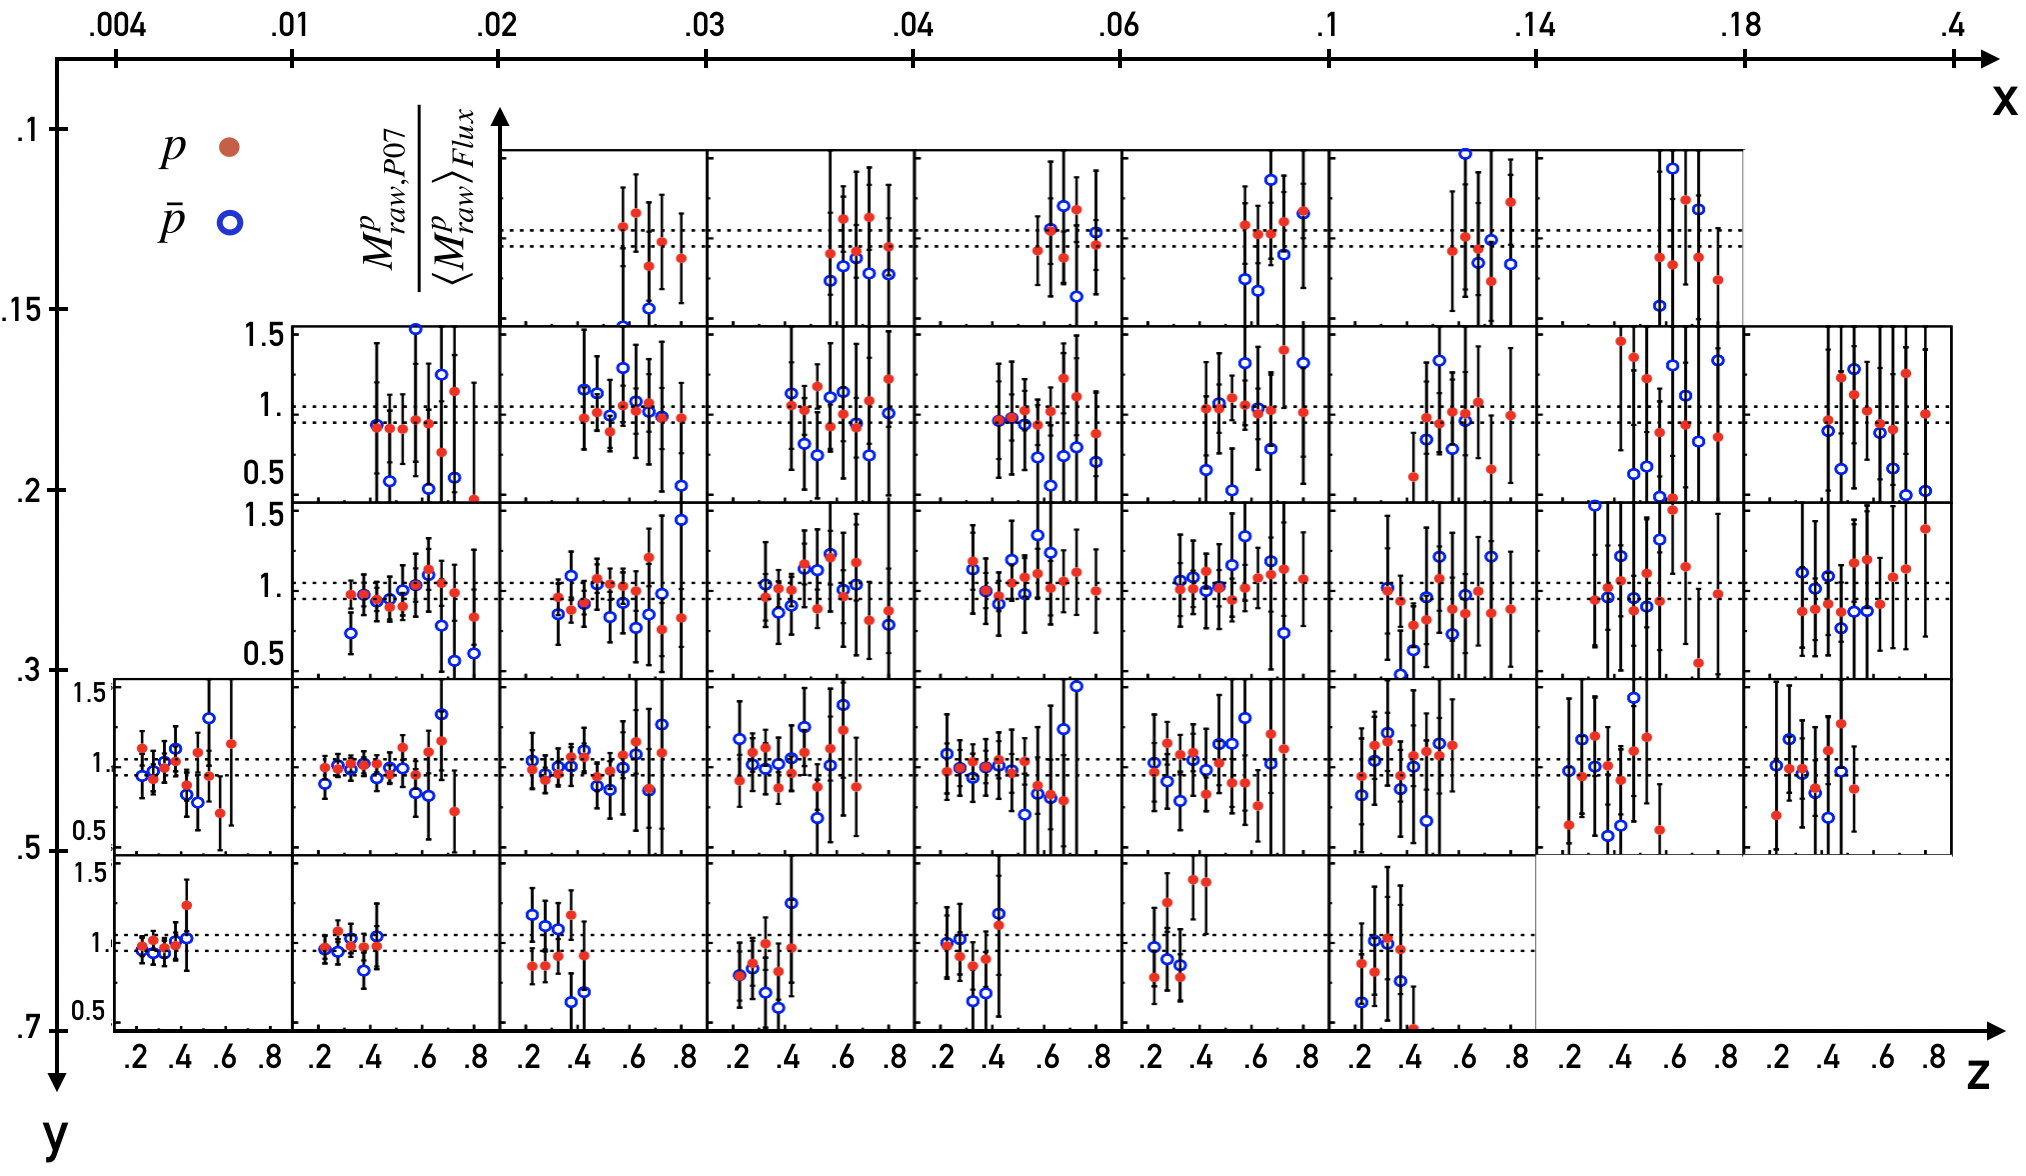
\includegraphics[scale=0.7]{./gfx/SysTimeMultp.png}
	\caption{Same as Fig. \ref{pic:hMultTime} but for proton multiplicities.}
	\label{pic:pMultTime}
\end{sidewaysfigure}

\newpage

%----------------------------------------------------------------------------------------

\section{Effect of the rescue procedure on the multiplcity sum}

\begin{figure}[!h]
  \centering
	\subfloat[]{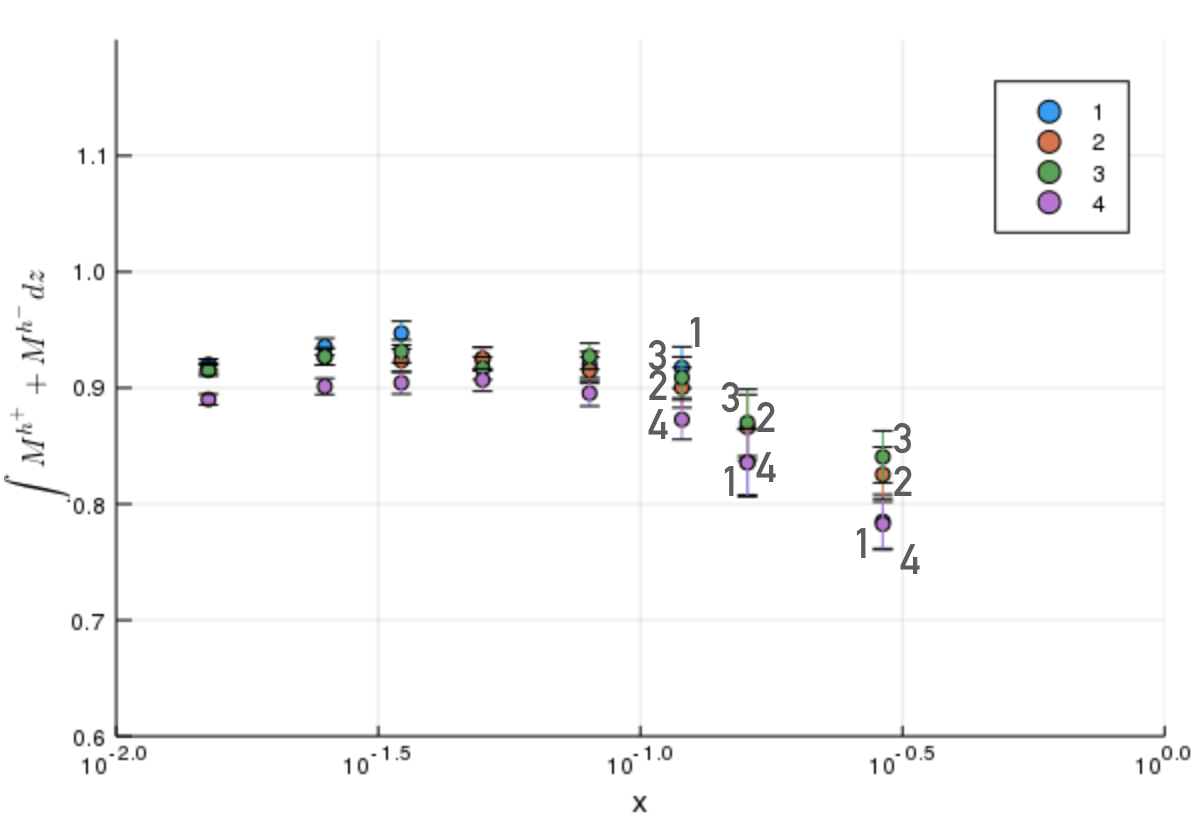
\includegraphics[scale=0.5]{./gfx/SumVertexB4RP.png}} \\
  \subfloat[]{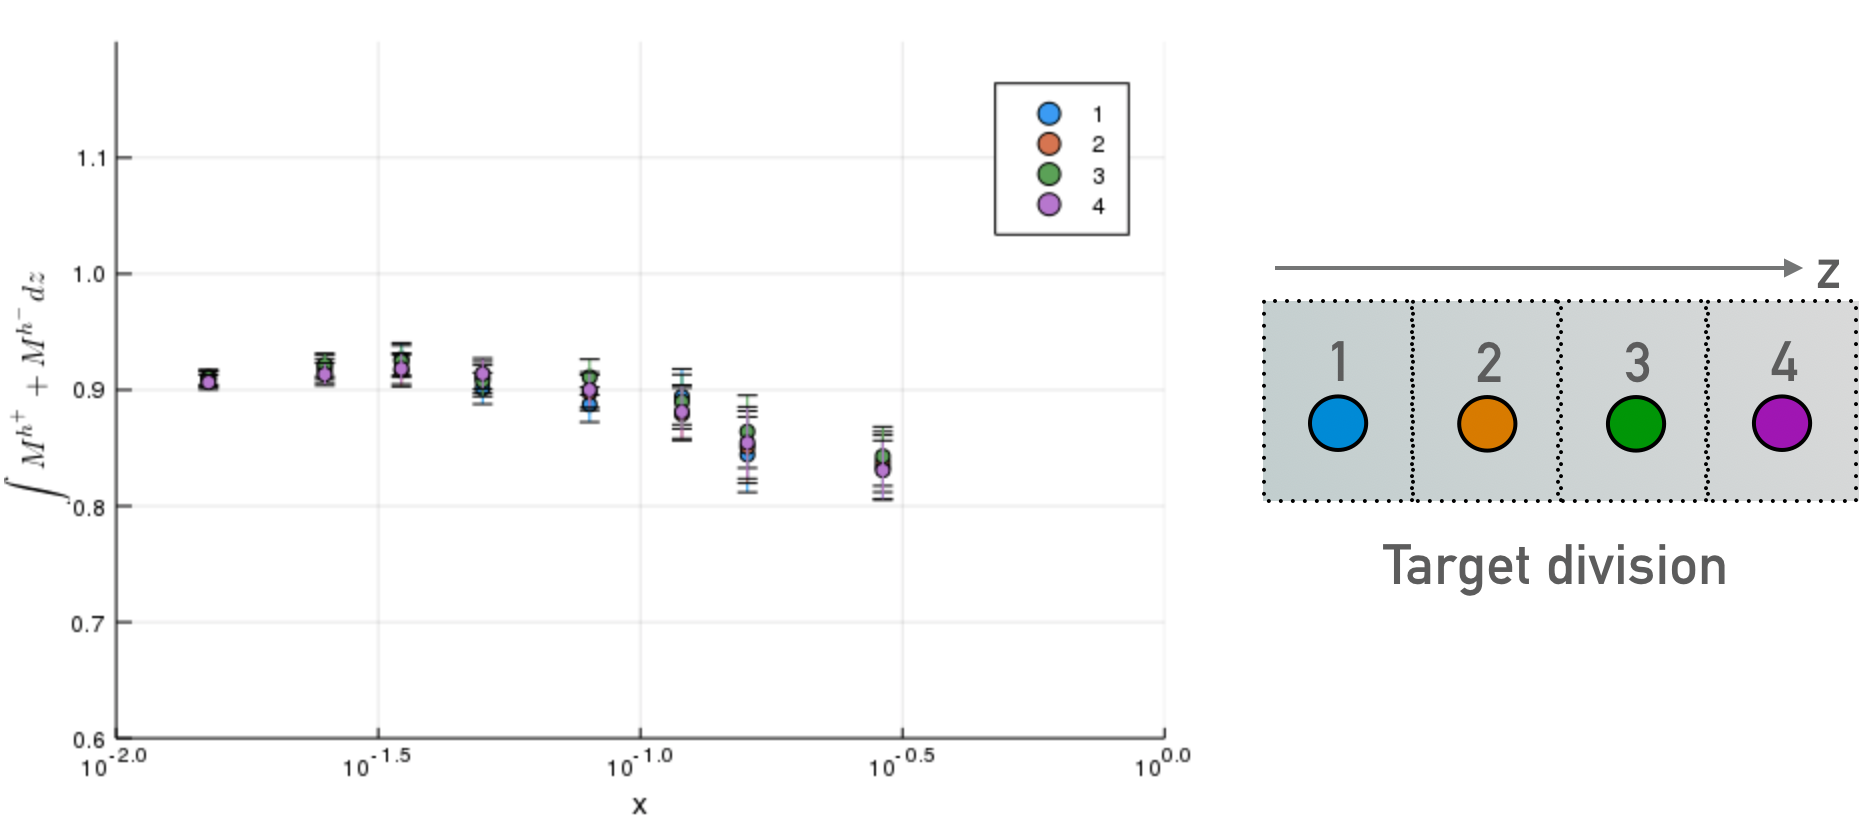
\includegraphics[scale=0.5]{./gfx/SumVertexBis.png}}
	\caption{Comparison of the multiplicity sum before the application  of the rescue procedure (a) and after (b) for different target slices.}
	\label{pic:Zvertexsum}
\end{figure}
